%%%%%%%%%%%%%%%%%%%%%%%%%%%%%%%%%%%%%%%%%%%%%%%%%%%%%%%%%%%%%%%%%%%%%%
% Documento PRINCIPAL da newsletter da Comissão de
% Pedometria da Sociedade Brasileira de Ciência do Solo
%
% NÃO EDITE ESSE ARQUIVO!
% 
% Language: Latex
% 
%%%%%%%%%%%%%%%%%%%%%%%%%%%%%%%%%%%%%%%%%%%%%%%%%%%%%%%%%%%%%%%%%%%%%%


% PREÂMBULO
\documentclass[a4paper]{report}

% Língua e codificação
\usepackage[brazilian]{babel}
\usepackage[utf8]{inputenc}
\usepackage[T1]{fontenc}

% para boot
\usepackage{amssymb,amsmath}

% Nota: é preciso incluir o pacote amsmath antes do pacote GRASSnews
% porque o último redefine o ambiente de equações...
\usepackage{GRASSnews}
\usepackage[round]{natbib}

% Figuras
\usepackage{graphicx}
\usepackage{wrapfig}

% para Sweave
\usepackage{listings}

% para tcltk-update
\usepackage{shortvrb}
%\usepackage{chapterbib}

\sloppy{}

% links
\usepackage[pdftex]{hyperref} % Deve ser o último pacote carregado
\hypersetup{colorlinks=true, citecolor=blue, linkcolor=blue, urlcolor=blue}

% DOCUMENTO
\begin{document}
 
% Edição da newsletter
\volume{1}
\volnumber{1}
\date{June 2004}
\titlepage



% Entrevista
\begin{article}
   \title{Entrevista}
\subtitle{com Paulo Ivonir Gubiani}
\maketitle
\begin{wrapfigure}{l}{0.15\textwidth}
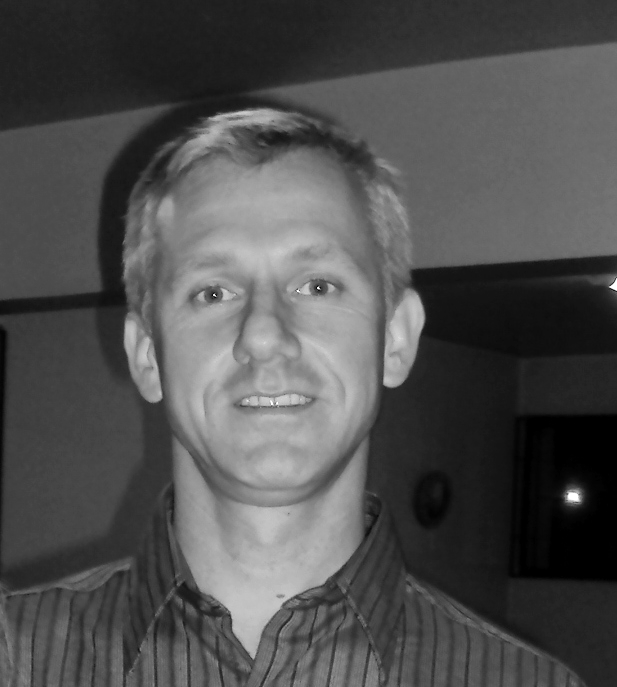
\includegraphics[width=0.15\textwidth]{figuras/foto-paulo}
\end{wrapfigure}

Nesta edição da \pedometria, entrevistamos o Professor Doutor Paulo Ivonir Gubiani para falar um pouco sobre sua experiência em modelagem matemática na área de Física do Solo, sua opinião com relação as pesquisas na área de modelagem, dificuldades e perspectivas futuras no Brasil. O Dr. Paulo atualmente é docente no Departamento de Solos - Setor de Física do Solo da Universidade Federal de Santa Maria (UFSM). Sua formação pós ensino médio foi realizada na UFSM, onde cursou Agronomia. Na mesma universidade fez seu mestrado e doutorado em Ciência do Solo na área de Processos Físicos e Morfogenéticos do Solo.

\pergunta{O que levou você a se interessar e estudar temas relacionados à modelagem matemática de dados ambientais, em especial, processos relacionados ao solo?}

\resposta{Paulo}{Penso que o estudo sobre modelagem matemática na área que atuo, isto é, Física do Solo, não é uma questão apenas de gosto ou interesse, mas sim de necessidade. O solo é um sistema aberto e dinâmico, e medidas pontuais de suas propriedades informam apenas estados do sistema. Na ciência, a medição constitui uma etapa fundamental, que é a observação. Porém, o ``fazer'' ciência vai muito além da observação. Em sistemas abertos e dinâmicos o principal interesse e função do pesquisador é conhecer a evolução do sistema no tempo, suas causas e consequências. As medições conseguem descrever o estado do sistema num instante de tempo, mas não permitem prever estados e consequências futuras. Com a modelagem matemática, estados do sistema podem ser simulados a partir do conhecimento da inter-relação de suas variáveis. A modelagem não visa substituir a medição, mas sim fornecer um valor aproximado para variáveis que, por razões técnicas ou físicas, não podem ser medidas (por exemplo, estado de um sistema no futuro). No que se refere ao solo, previsões aproximadas de erosão do solo, estoque de carbono, transferência de compostos abióticos e bióticos entre ambientes, armazenamento de água no solo, emissão de gases de efeito estufa, entre outros, são de grande utilidade para que cientistas do solo projetem as consequências para a humanidade do atual modo de utilização do solo. A modelagem é, certamente, uma simplificação de um sistema real. Contudo, ela é uma simplificação integradora. Quando modelamos, conectamos os componentes de um sistema e analisamos o sistema como um todo a partir das relações naturalmente indissociáveis de seus componentes. Quando não modelamos, simplificamos ainda mais o sistema, limitamos e tornamos mais falíveis as previsões sobre o comportamento do sistema.}

\pergunta{Quais os projetos de pesquisa que você está desenvolvendo ou participando relacionados à modelagem e estimação de propriedades do solo ou processos que ocorrem no solo?}

\resposta{Paulo}{No momento, estou participando diretamente de um estudo de dissertação sobre modelagem da infiltração de água no solo. Nosso objetivo é desenvolver uma aplicação numérica do modelo de Green-Ampt para perfil de solo multicamada, sem limitação do número de camadas de solo com distintas propriedades hidráulicas e sob condições de chuva natural. O estudo está na fase de obtenção de dados. As primeiras simulações com o algoritmo que criamos são promissoras, mas precisamos de mais medições para avaliação e calibração do modelo. Também auxilio uma doutoranda do Programa de Pós-Graduação em Engenharia Agrícola da UFSM, na implementação de modelos de balanço hídrico do solo, no modelo de simulação de produção da cultura da mandioca que ela está desenvolvendo.}

\pergunta{Qual sua opinião a respeito do cenário atual das pesquisas em modelagem na ciência do solo no Brasil?}

\resposta{Paulo}{Minha opinião sobre essa questão é baseada em duas análises. A primeira foi feita pelo professor Quirijn de Jong Van Lier, do CENA/USP, e foi apresentada em sua palestra no XXXIII Congresso Brasileiro de Ciência do Solo, na cidade de Uberlândia-MG, em 2011. O professor Quirijn analisou a frequência de ocorrência dos termos ``modelo'' ou ``modelagem'' nos títulos das publicações da área de física do solo em três fontes: nos resumos do XXXII Congresso Brasileiro de Ciência do Solo de 2009 (XXXII CBCS); na Revista Brasileira de Ciência do Solo (RBCS), no período de 2003 a 20011; e na Soil Science Societe American Journal (SSSAJ), no período de 2006 a 2011. Sua constatação foi que os termos ``modelo'' ou ``modelagem'' raramente apareciam nos títulos das publicações do XXXII CBCS, apareciam em menos que 5 por cento dos títulos da RBCS e em torno de 10 por centodos títulos da SSSAJ. Além disso, a comparação entre RBCS e SSSAJ demonstrou que nos dedicamos pouco ao estudo de processos e instrumentação, assuntos que antecedem e dão suporte para a modelagem. A segunda análise foi um levantamento que eu fiz também da frequência de ocorrência dos termos ``modelo'' ou ``modelagem'' nos títulos dos 221 resumos apresentados no XXXIV Congresso Brasileiro de Ciência do Solo de 2013, na comissão de física do solo. Apenas em três dos 221 títulos constava o termo ``modelagem'' (\url{http://gubianisolos.blogspot.com.br/2013/08/fisica-do-solo-apresentada-no-xxxivcbcs.html}). Esse panorama da modelagem para a Ciência do Solo no Brasil poderia ser refinado por pesquisador, usando os títulos de seus artigos cadastrados na plataforma Lattes. Caso isso fosse feito, verificaríamos que existem alguns pesquisadores que atuam com maior ênfase na modelagem em relação a outros muitos que ainda não iniciaram ou estão iniciando estudos com esse propósito.}
\vspace{5mm}
\begin{figure}[h!]
 \centering
 \includegraphics[width=0.8\textwidth]{figuras/foto-paulo-mensuration}
 \caption{Monitoramento da umidade do solo pela técnica da Reflectometria no Domínio do Tempo (TDR). Tal técnica é comumente utilizada em estudos de modelagem matemática na área de Física do Solo. Fonte: Paulo Gubiani.}
\end{figure}

\pergunta{Qual a sua opinião a respeito de assuntos como a modelagem matemática de processos e atributos do solo, geoestatística e linguagem de programação como disciplinas nos cursos de Pós-Graduação da área de solos no Brasil?}

\resposta{Paulo}{Penso que a inclusão desses conteúdos como disciplinas nos cursos de Pós-Graduação (PG) da área de solos está diretamente relacionada com o resultado técnico-científico que cada PG vislumbra e com a independência dessa produção de PG externos. Para um PG cujos professores orientadores praticam a modelagem matemática, essas disciplinas, ou algumas delas, já são ofertadas aos estudantes, porque esses conteúdos são indispensáveis para o desenvolvimento da modelagem matemática. Para um PG cujos professores orientadores não praticam a modelagem matemática, e que têm interesse em atuar nessa área, essas disciplinas teriam que ser cursadas também pelos professores. É pouco provável que alguém queira orientar uma pesquisa sobre modelagem matemática se não domina o assunto. Outro agravante é a combinação do precário embasamento matemático de estudantes de graduação que ingressam na pós-graduação em ciência do solo e o curto período de tempo que esses estudantes têm no mestrado e no doutorado para que disciplinas oferecidas na pós-graduação supram as carências e adicionem os requisitos matemáticos mínimos para a modelagem. Embora existam exceções, na maioria dos casos o que se consegue nessa condição de carência de formação é habilitar operadores de softwares de modelagem. Isso é útil para formar e/ou exportar operadores de softwares executores de simulações. Mas, se os PGs vislumbram gerar e exportar modelos, então acredito que, além de ofertar disciplinas na pós-graduação, é essencial o fortalecimento da formação matemática, estatística e de programação na graduação e, sobretudo, nos grupos de pesquisa durante a iniciação científica.}

\pergunta{Pela sua experiência na área de modelagem ambiental, quais as principais dificuldades e desafios encontrados para os pesquisadores brasileiros desenvolverem seus trabalhos nessa área?}

\resposta{Paulo}{Minha experiência é bem pequena se comparada à experiência de pesquisadores que trabalham com modelagem há bastante tempo. Porém, o que tenho sentido e notado até o momento coincide com a opinião de pesquisadores experientes no assunto. Sabe-se que o pesquisador ou seu grupo deve estar munido das habilidades necessárias para a modelagem. Nesse ponto, ele deve compreender bem conceitualmente o sistema físico que quer modelar, conhecer ou desenvolver possibilidades matemáticas para descrição das relações dos componentes do sistema e conectar toda a estrutura matemática numa unidade que permite a reprodução aproximada do sistema. Além disso, os pesquisadores devem efetuar a calibração e validação dos seus modelos, o que exige medições no sistema que está sendo modelado. Os desafios principais dependem do sistema que está sendo modelado. Pode ser a formação matemática e de programação (quando se quer criar ou modificar um modelo existe) a formação de equipes multidisciplinares (modelagem de sistemas multicompartimentais) ou a formação de grupo de pesquisa e aquisição de equipamentos (monitoramento para medições de sistemas multicompartimentais e espacialmente abrangentes). Do ponto de vista da capacitação, a maioria dos estudantes nas universidades tem um computador pessoal, ferramenta que facilita o aprendizado de modelagem matemática. Porém, a popularização do computador é recente no Brasil. Além disso, os estudantes dos cursos de graduação que mais candidatos oferecem para a pós-graduação em ciência do solo, embora tenham a ferramenta computacional, dispõem de pouco ou nada de disciplinas sobre modelagem matemática e programação. Outro grande desafio é externo ao escopo da modelagem. Trata-se da motivação da produção de dissertações, teses e artigos científicos num modelo que prevalece o critério da quantidade. Logicamente se produz em maior quantidade quanto mais simples de serem executadas forem as pesquisas. A modelagem se ocupa em explicar sistemas, o que requer a descrição de processos, trabalho que é bem mais complexo do que medir e discutir relações entre propriedades num período pequeno de tempo. Fazendo uma analogia à expressão ``publique ou pereça'', usada para indicar a atual situação da ciência, basta fazer uma consulta nos currículos Lattes dos pesquisadores que se perceberá claramente que os pesquisadores ``perecem'' com a modelagem e ``publicam'' com a relação estatística de propriedades.}

\pergunta{Qual a sua opinião a respeito da interdisciplinaridade nos grupos de pesquisa da área de solos para desenvolver trabalhos que contribuam para meio científico? Em sua opinião, existe interdisciplinaridade nos grupos de pesquisa do Brasil? Sim ou Não? Por quê?}

\resposta{Paulo}{O conceito de interdisciplinaridade ainda segue em construção e está sujeito a interpretações distintas, como mobilização dos conteúdos de duas ou mais disciplinas, fusão de conteúdos de disciplinas em uma nova, etc. O primeiro caso é o que mais acontece nos grupos de pesquisa, com intensidade e abrangência variável. A solução de problemas simples depende menos da mobilização de conhecimentos de várias disciplinas, ao passo que problemas complexos se inserem num escopo interdisciplinar. Porém, qualquer conhecimento novo é uma contribuição importante da ciência para ampliar o corpo de conhecimentos existente e não somente os que resultam de interação interdisciplinar. A prática da interdisciplinaridade vai avançando na medida em que os grupos se consolidam, os projetos de pesquisa passam a tratar de problemas mais abrangentes, necessitam e reúnem conhecimentos de várias áreas, recebem mais suporte financeiro e estrutural e consolidam parcerias nacionais e internacionais. Nos últimos anos, interações e cooperações aumentaram, tanto em nível nacional como internacional (verificar a seção acesso à informação no site da CAPES) o que cria espaço para a mobilização de conteúdos de várias disciplinas para a solução de problemas. Há vários exemplos no Brasil da prática interdisciplinar resultante dessas interações, como a formação de grupos de estudo dos sistemas integrados lavoura-pecuária ou lavoura-pecuária-floresta, grupos de estudo de processos hidrossedimentológicos em escala de bacia hidrográfica e grupos dedicados ao mapeamento digital de solo. Nesses estudos, o que guia o pesquisador é a noção holística e sistêmica, de integração dos componentes de um sistema, do estudo do todo a partir de suas partes. Ainda há muito trabalho acadêmico para ser feito para que essas e muitas outras áreas de conhecimento sejam cobertas com pesquisas integradoras. Para esse propósito, incentivar estudantes a aprenderam modelagem matemática é uma ótima iniciativa para exercitar essa noção integradora e interdisciplinar.}
%%% Local Variables:
%%% mode: latex
%%% TeX-master: 4rd-edition.tex
%%% End:
\end{article}



% Artigos em geral
\begin{article}
   %%%%%%%%%%%%%%%%%%%%%%%%%%%%%%%%%%%%%%%%%%%%%%%%%%%%%%%%%%%%%%%%%%%%%%
% Modelo de ARTIGO GERAL da newsletter da Comissão
% de Pedometria da Sociedade Brasileira de Ciência do Solo
%
% Esse modelo deve ser utilizado para a construção de ARTIGOS GERAIS.
% 
% Recomendações gerais:
% A edição desse documento deve ser feita utilizando um editor LaTeX
% como o RStudio.
% Linhas precedidas por '%' não precisam ser deletados pois não
% são reconhecidos durante a copilação do documento.
% Elementos como '\title{}' constituem comandos e não devem
% ser alterados, exceto o conteúdo entre parênteses.
% Ex.: '\title{Título do seu artigo}' = '\title{O que é Pedometria?}'
%
% Coloque seu nome como nome do arquivo. Ex. 'artigo-alessandro.tex'.
% O arquivo final deve ser enviado compactado junto das figuras.
%
% Language: Latex
%%%%%%%%%%%%%%%%%%%%%%%%%%%%%%%%%%%%%%%%%%%%%%%%%%%%%%%%%%%%%%%%%%%%%%

% Cabeçalho do seu artigo. Substitua apenas as informações entre parênteses.
\title{Título do seu artigo}
\subtitle{Subtítulo do seu artigo}
\author{por primeiro autor e segundo autor}
\maketitle



% Aqui vai a sua foto. Não adicione o caminho, apenas o nome do
% arquivo e o formato.
\begin{wrapfigure}{l}{0.15\textwidth}
\includegraphics[width=0.15\textwidth]{sua-foto-aqui.jpg}
\end{wrapfigure}



% Aqui começa seu texto.
Era uma vez...



% Se você tiver seções use os comandos a seguir. Do contrário,
% simplesmente apague-os.
\subsection{Título da sua subseção}
\label{subsec:rótulo-da-sua-subseção}



% Aqui você continua seu texto.
Era uma vez...



% Com os comandos abaixo você insere uma figura.
\begin{figure}[htbp]
   \centering
   % aqui vocÊ identifica o aquivo no formato PNG ou PDF:
   \includegraphics[scale=0.8]{sua-figura-aqui.jpg}

   % aqui você dá um título à figura:
   \caption{Esse é o título da miha figura.}

   % e aqui você define o rótulo da figura, que é usado para criar
   % links no documento com a função '\ref{}':
   \label{fig:rótulo-da-figura}
\end{figure}



% Aqui você continua seu texto.
E para citar a figura use o comando \ref{fig:rótulo-da-figura}.



% Se você tiver mais uma seção, use os comandos a seguir. Do
% contrário, simplesmente apague-os.
\section{Nome da minha outra seção}
\label{sec:rótulo-da-minha-outra-seção}



% Aqui você continua seu texto.
Era uma vez...



% Para adicionar linhas de comando de algum software, use a 
% função 'smallverbatim':
\begin{smallverbatim}
# cole aqui seu comando:
GRASS 5.7.-cvs:~ > d.mon x0
using default visual which is TrueColor
ncolors: 65536
Graphics driver [x0] started
GRASS 5.7.-cvs:~ > d.rast wcm
 100%
GRASS 5.7.-cvs:~ >

etc. 
\end{smallverbatim}



% Aqui você continua seu texto.
Era uma vez...



% Se você quiser citar alguma referência bibliográfica use a função
% '\cite{nome:ano}' e '\citep{nome:ano}'. Por exemplo:
Os resultados de \cite{highlander:2003} são contraditórios.



% Se a citação deve aparecer entre parêntese, então use o seguinte:
Os resultados são contraditórios \citep{highlander:2003}.



% Aqui termina o seu texto e começa a sua lista de referências
% bibliográficas.
\begin{footnotesize}
\begin{thebibliography}{99}



% primeiro item da sua lista:
% a primeira linha descreve como a citação aparece no texto
\bibitem[Highlander et~al. (2003) Highlander, Batman, Wolverine, Hulk]{highlander:2003}
% essas três linhas definem como a citação aparece nas referências
L.M. Highlander, M.G. Batman, A.S. Wolverine, S.P. Hulk (2003)
\newblock A pedometria é muito legal.
\newblock {\em Revista Pedometria} 24: 69-96.



% copie e edite as linhas acima para adicionar mais referências


\end{thebibliography}
\end{footnotesize}
% aqui termina sua lista de referências!



% aqui vão as suas informações
\address{Seu Nome\\
  Sua Organização\\
  \url{seu website}\\
  \email{seu endereço de e-mail}}



%%% Local Variables: 
%%% mode: latex
%%% TeX-master: documento-principal.tex
%%% End: 


\end{article}



% Artigo sobre novas publicações
\begin{article}
   \title{Novas publicações em pedometria}
\maketitle
\begin{wrapfigure}{l}{0.15\textwidth}
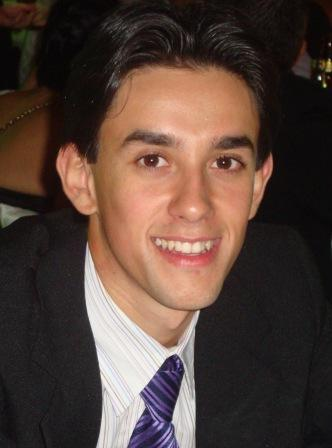
\includegraphics[width=0.15\textwidth]{figuras/foto-jean}
\end{wrapfigure}
O segundo número da nossa \textit{Newsletter} inaugura a seção de divulgação de novas publicações em pedometria. Todos podem contribuir enviando informações básicas sobre novas publicações, sejam elas nacionais ou internacionais. Basta enviar a contribuição ao editor responsável pela seção de novas puvlicações em pedometria, Jean Michel Moura-Bueno, pelo endereço de e-mail \email{bueno.jean1@gmail.com}.\\
As contribuições deverão ser sucintas, com tamanho inferior ao de um resumo geralmente apresentado em artigos científicos. Como estas contribuições servirão como propagandas de novos trabalhos publicados, é recomendado apresentar apenas informações chave, destaques que realmente chamam a atenção do leitor. Uma bom exemplo para ser seguido são os \emph{highlights} usados nos artigos da Elsevier: \emph{Os ``highlights'' são um pequeno conjunto de pontos que transmitem os resultados principais e fornecem aos leitores uma visão textual rápida do artigo}. Os resumos originais não serão publicados na \textit{Newsletter} por tal prática envolver questões de direitos dos autores e editoras das publicações originais.\\
Também é importante apresentar a forma de citação recomendada pelos autores, bem como o endereço da publicação na internet. Caso a publicação possua alguma figura interessante e autoexplicativa, a mesma deve ser enviada juntamente com o texto descritivo para a \textit{Newsletter}.
\section{Exemplo}
Abaixo há um exemplo utilizando uma publicação recente. Primeiro, é mostrado o resumo do artigo publicado no periódico científico e, em seguida, o formato recomendado para publicação na seção de novas publicações em pedometria da nossa \textit{Newsletter}.
\subsection{Título da publicação}
Building predictive models of soil particle-size distribution
\subsection{Citação}
A. Samuel-Rosa, R.S.D. Dalmolin, P. Miguel (2013) Building predictive models of soil particle-size distribution. {\em Revista Brasileira de Ciência do Solo} 37:422-430.
\subsection{Resumo original - não será publicado}
É possível construir modelos preditivos (MPs) da distribuição do tamanho de partículas do solo (DTP) em uma região que possua geologia complexa e uma superfície geomórfica jovem e instável? O principal objetivo deste trabalho foi responder a essa questão. Um conjunto de 339 amostras de solo de uma pequena bacia hidrográfica de encosta do sul do Brasil foi usado para construir MPs da DTP na camada superficial do solo. Modelos de regressão linear múltiplos foram construídos com atributos de terreno (elevação, declividade, área de captação, índice de convergência, índice de umidade topográfica). Os MPs explicaram mais da metade da variância dos dados. Esse desempenho é semelhante (se não melhor) ao da abordagem tradicional de mapeamento de solos. Para algumas frações de tamanho, o desempenho dos MPs pode chegar a 70\%. As maiores incertezas ocorrem nas áreas de maior complexidade geológica. Assim, melhorias significativas nas predições somente poderão ser alcançadas se dados geológicos acurados forem 
disponibilizados. Enquanto isso, MPs construídos a partir de atributos de terreno são eficientes em estimar a DTP de solos de regiões com geologia complexa.
\subsection{Resumo para a \textit{Newsletter}}
É possível construir modelos preditivos da distribuição do tamanho de partículas numa região com geologia complexa (arenitos e basaltos com arenito \emph{intertrap}) e superfície geomórfica jovem e instável? Esta é a pergunta que nos fez desenvolver este estudo em uma pequena bacia hidrográfica no RS. Com um conjunto de $n=339$ observações e alguns atributos de terreno, construímos modelos lineares para predizer a distribuição do tamanho de partículas na camada superficial do solo, tratados como dados composicionais. Os resultados sugerem que o desempenho dos modelos pode ser inferior, similar ou superior ao método tradicional de mapeamento do solo. As maiores incertezas estão conectadas às áreas onde as informações geológicas são mais pobres. Destacamos que a qualidade dos mapas geológicos deve ser melhorada se predições superiores forem demandadas.
\begin{footnotesize}
\begin{thebibliography}{99}
\bibitem[Samuel-Rosa et~al. (2013) Samuel-Rosa, Dalmolin, Miguel]{Samuel-RosaEtAl:2013} 
A. Samuel-Rosa, R.S.D. Dalmolin, P. Miguel (2013)
\newblock Building predictive models of soil particle-size distribution.
\newblock {\em Revista Brasileira de Ciência do Solo} 37:422-430. [\url{http://dx.doi.org/10.1590/S0100-06832013000200013}]
\end{thebibliography}
\end{footnotesize}
\address{Jean Michel Moura-Bueno\\
  Universidade Federal de Santa Maria\\
  \email{bueno.jean1@gmail.com}}
%%% Local Variables: 
%%% mode: latex
%%% TeX-master: documento-principal.tex
%%% End: 
\end{article}



% Artigo de eventos
\begin{article}
   \title{Eventos}
\maketitle


\section{INTERGEO}
\subsection{Istambul, Turquia, 28-29/4/2014}
O congresso é organizado pela German Society of Geodesy, Geoinformation and Land Management (DVW). 
Maiores informações podem ser encontradas no endereço \url{http://www.intergeo-eurasia.net/en/index.html}.


\section{Conferência e Feira de Geomática e Soluções Geoespaciais}
\subsection{São Paulo, Brasil, 7-9/5/2014}
O evento é organizado por MundoGEO.
Maiores informações podem ser encontradas no endereço \url{http://mundogeoconnect.com/2014/}.


\section{ISRIC'S Spring School 2014}
\subsection{Wageningen, Holanda, 12-16/5/2014}
O evento é organizado pelo International Soil Reference and Information Centre - ISRIC. Serão abordados temas relacionados ao Mapeamento Digital de Solos (MDS) e uso de softwares para análise de dados de solos.
Maiores informações podem ser encontradas no endereço \url{http://www.isric.org/content/isrics-spring-school-2014}.


\section{20th Word Congress of Soil Science}
\subsection{Jeju, Korea, 8-13/06/2014}
O congresso é organizado pela International Union of Soil Sciences (IUSS). 
Maiores informações podem ser encontradas no endereço \url{http://www.20wcss.org/}.


\section{12th International Conference of Precision Agriculture}
\subsection{Sacramento, Califórnia (USA), 20-23/07/2014}
O congresso é organizado pela Sociedade Internacional de Agricultura de Precisão.
Maiores informações podem ser encontradas no endereço \url{https://www.ispag.org/ICPA/}.


\section{XX Congresso Latinoamericano de la Ciencia Del Suelo}
\subsection{Cusco, Perú, 9-15/11/2014}
O evento é organizado pela Sociedade Latinoamericana de Ciência do Solo (SLCS).
Maiores informações podem ser encontradas no endereço \url{http://www.xxcongresolatinoamericanodesuelosperu.org/programa.php}.


\section{6th Global Workshop on Digital Soil Mapping}
\subsection{Nanjing, China, 11-14/11/2014}
O evento é  organizado pelo Instituto de Ciência do Solo da Academia Chinesa de Ciências. O prazo para submissão de trabalhos é 31/07/2014.
Maiores inforamçoes podem ser encontradas no endereço \url{http://dsm2014.csp.escience.cn/}.


\address{Jean Michel Moura-Bueno\\
    Universidade Federal de Santa Maria\\
    \email{bueno.jean1@gmail.com}}
\end{article}



% Artigo de instrução aos autores
\begin{article}
   \title{Instruções aos autores}
\maketitle
\newcommand{\SBCS}{\href{http://www.sbcs.org.br/}{SBCS}}
\newcommand{\Nature}{\href{http://www.nature.com/nature/authors/gta/}{Nature}}
\newcommand{\Science}{\href{http://www.sciencemag.org/about/authors}{Science}}
\newcommand{\CreativeCommons}{\href{http://creativecommons.org/licenses/by-sa/2.0/}{CC-BY-SA}}
\newcommand{\Kile}{\href{http://kile.sourceforge.net/}{Kile}}
\newcommand{\MiKTeX}{\href{http://miktex.org/}{MiKTeX}}
\newcommand{\aquiLaTeX}{\href{https://docs.google.com/document/d/1F3IXzWNCeUrwKeFxA4iHS3aw1nforK1IqB126xbawvA/edit?usp=sharing}{aqui}}
\newcommand{\aquiWord}{\href{https://docs.google.com/document/d/1pyK03RBDPhOMrTVfvj9NcEfjGWeswqYbYDqEKq83drQ/edit?usp=sharing}{aqui}}
\newcommand{\Geoderma}{\href{http://www.elsevier.com/author-schemas/latex-instructions}{Geoderma}}
\newcommand{\EJSS}{\href{http://onlinelibrary.wiley.com/journal/10.1111/\%28ISSN\%291365-2389/homepage/ForAuthors.html}{European Journal of Soil Science}}

\subsection{Escopo e política}

\pedometria{} é a \textit{Newsletter} (boletim técnico-científico) da Comissão de Pedometria da Sociedade Brasileira de Ciência do Solo (\SBCS). Assim sendo, dedica-se à publicação de artigos relacionados à aplicação de métodos matemáticos e estatísticos para o estudo da gênese e distribuição dos solos, o que abrange desde discussões conceituais até a aplicação prática de sensores e modelos. Especificamente, os seguintes tópicos costumam ser cobertos:

\begin{itemize}
 \item explicitação de conceitos pedométricos;
 \item entrevista com pedometrista;
 \item opinião sobre tema pedométrico relevante;
 \item descrição de equipamentos e sensores remotos;
 \item descrição de softwares e suas funcionalidades;
 \item eventos técnico-científicos;
 \item expressão artística em pedometria;
 \item novas publicações científicas em pedometria.
\end{itemize}

Os artigos submetidos para publicação em \pedometria{} NÃO DEVEM ser formais como aqueles geralmente submetidos para revistas científicas tradicionais da área de pedometria. DEVE-SE usar linguagem CLARA e INFORMAL, preferencialmente na VOZ ATIVA. O uso da voz ativa é uma recomendação para publicação em ambas as revistas \Nature{} e \Science:

\begin{description}
 \item \textit{Nature} ``Nature journals like authors to write in the active voice (`we performed the experiment...') as experience has shown that readers find concepts and results to be conveyed more clearly if written directly.''
 \item \textit{Science} ``Use active voice when suitable, particularly when necessary for correct syntax (e.g., `To address this possibility, we constructed a lZap library ...,' not `To address this possibility, a lZap library was constructed...').''
\end{description}

Conceitos pedométricos devem ser introduzidos com SENSIBILIDADE, tendo em mente que os leitores podem os desconhecer e/ou não possuir base conceitual suficiente para compreendê-los em uma única leitura. A estrutura do artigo deve ser concebida da mesma maneira que o fazemos para contar uma história a um amigo ou familiar, a fim de cativar o leitor e envolvê-lo no emocionante universo da pedometria. Caso a comissão editorial entenda que a compreensão do texto exija aprofundado conhecimento prévio do leitor, os autores serão solicitados a torná-lo mais simples e amigável.

O escopo e política de \pedometria{} coloca-a como veículo de divulgação e desmistificação da pedometria no Brasil. Trata-se de uma publicação com três edições anuais que permite aos pesquisadores brasileiros divulgar suas pesquisas pedométricas e, sobretudo, conhecerem uns aos outros. Isso é importante porque, assim como a própria pedometria, a maioria dos pedometristas também são bastante jovens, muitos dos quais ainda estão desenvolvendo seus estudos de mestrado e/ou doutorado. Por este motivo, \pedometria{} é distribuída gratuitamente via Internet, estando registrada sob a licença Creative Commons Atribuição-Compartilha Igual 3.0 Não Adaptada (\CreativeCommons).\\
\\
\begin{figure}[h!]
 \centering
 
\includegraphics[width=0.8\textwidth]{figuras/cc-by-sa}
 \caption{Licença Creative Commons Atribuição-Compartilha Igual 3.0 Não Adaptada.}
\end{figure}

\subsection{Estrutura do artigo}

A estrutura do artigo é inteiramente definida pelo(s) autor(es). Sugere-se que sejam utilizadas subdivisões em até dois níveis de profundidade (seções e subseções), não necessariamente definidas como em artigos científicos tradicionais. Os artigos podem ter, além do título, um subtítulo. Resumo e palavras-chave não são utilizados.

\subsubsection{Figuras e tabelas}

Figuras e tabelas são recomendadas, sendo uma foto do(s) autor(es) obrigatória. Figuras devem ser preparadas no formato PNG, com resolução mínima de 300 dpi.

\subsubsection{Referências bibliográficas}

Referências bibliográficas não são mandatórias, sobretudo no caso de artigos apresentando a opinião do autor sobre um tema pedométrico. Caso citações sejam feitas ao longo do texto, a lista de referências deve ser organizada na ordem em que as citações são feitas no texto. Importante notar que o estilo de citação numérica sobrescrita da \textit{Nature} é utilizado.

A lista de referências bibliográficas deve conter até cinquenta itens. O conteúdo da lista de referências deve ser econômico, incluindo apenas informações fundamentais para a sua identificação. Artigos, trabalhos em anais de eventos ou em coleções, e trabalhos publicados em veículos periódicos similares, devem ser formatados da seguinte maneira:

\vspace{0.5cm}
\noindent{A.B. McBratney, M.L. Mendonça-Santos, B. Minasny (2003) On digital soil mapping. \textit{Geoderma}, 117:3-52. \doi{10.1016/S0016-7061(03)00223-4}}
\vspace{0.5cm}

\noindent{onde \textit{link} refere-se ao endereço na Internet onde o referido documento pode ser encontrado. No caso de artigos científicos recomenda-se utilizar o Digital Object Identifier (\href{http://www.doi.org/}{DOI}). Livros, teses, dissertações, relatórios e outros meios de publicação não periódicos devem ser formatados da seguinte maneira:}

\vspace{0.5cm}
\noindent{H. Jenny (1994) \textit{Factors of soil formation - a system of quantitative pedology}. Toronto: Dover Publications.}
\vspace{0.5cm}

\noindent{Caso as publicações não periódicas estejam disponíveis na Internet, um link deve ser adicionado assim como para as publicações periódicas.}

\subsection{Preparo do artigo}

Os artigos podem ser preparados utilizando processadores de texto tradicionais, como por exemplo o MS Office Word (*.doc) e o LibreOffice Writer (*.odt), ou a linguagem de marcação \LaTeX() (*.tex). Preferência deve ser dada ao formato \LaTeX() sempre que possível a fim de facilitar o trabalho da equipe editorial. Documentos no formato PDF não são aceitos.

\subsubsection{Word ou Writer}

Um modelo para preparo do artigo usando processadores de texto tradicionais pode ser acessado clicando \aquiWord.

\subsubsection{\LaTeX}

\href{http://pt.wikipedia.org/wiki/Latex}{\LaTeX} é uma \href{http://pt.wikipedia.org/wiki/Linguagem_de_marca\%C3\%A7\%C3\%A3o}{linguagem de marcação} amplamente utilizada para a produção de textos matemáticos e científicos devido à sua alta qualidade tipográfica. Utilizar uma linguagem de marcação para elaboração de textos constitui no uso de comandos escritos para definir a formatação do documento, ao contrário dos editores tradicionais que oferecem abas e caixas de diálogo para clicar e definir parâmetros de formatação. Na prática, ao produzir um texto em \LaTeX, o autor não vê o produto final formatado na tela do computador imediatamente, mas apenas o texto e os comandos de formatação. O objetivo é distanciar o autor o máximo possível da apresentação visual do artigo, ou seja, ao invés de trabalhar com ideias visuais, o autor é encorajado a trabalhar com conceitos lógicos independentes da apresentação final do artigo. Além disso, linguagens de marcação como o \LaTeX{} permitem agilizar a confecção do documento final (PDF) e reproduzir o conteúdo em outros formatos para apresentação em meio digital como o html. Atualmente, importantes revistas científicas da área de pedometria adotam o \LaTeX{} para a confecção de seus artigos, como por exemplo \Geoderma{} e \EJSS.

Apesar de diferente dos processadores de texto tradicionais, usar \LaTeX{} é bastante fácil, sendo necessário apenas compreender a sua lógica de funcionamento. Para isso é bom dar uma olhada no \href{http://www.stdout.org/~winston/latex/}{Manual Rápido \LaTeX{}} para conhecer alguns comandos básicos. O preparo dos artigos usando \LaTeX{} pode ser feito usando softwares como Bloco de Notas, WordPad, e Gedit. Entretanto, é mais aconselhado usar um software específico para a edição de documentos em \LaTeX, como o \Kile{} e o \MiKTeX. Tais softwares auxiliam a inserção dos comandos necessários para a formatação do texto sem a necessidade de memorizá-los.

Um modelo para preparo do artigo usando \LaTeX{} pode ser acessado clicando \aquiLaTeX.

\subsection{Submissão}

Qualquer pessoa pode submeter um artigo para publicação em \pedometria{} sem qualquer custo. Quando o artigo estiver pronto, adicione todos os arquivos utilizados (inclusive as figuras originais) à uma pasta comprimida e envie para a comissão editorial usando o endereço de e-mail \email{pedometria.news@gmail.com}.

\subsection{Comissão editorial}

Alessandro Samuel-Rosa\\
\textit{ISRIC - World Soil Information}\\
\textit{Wageningen University and Research Center}\\
\email{alessandro.rosa@wur.nl}\\
\\
André Geraldo de Lima Moraes\\
\textit{Curso de Pós-Graduação em Agronomia-Ciência do Solo}\\
\textit{Universidade Federal Rural do Rio de Janeiro}\\
\email{andrehmuz@hotmail.com}\\
\\
Diego Silva Siqueira\\
\textit{Grupo de Pesquisa Caracterização do Solo para fins de Manejo Específico}\\
\textit{Universidade Estadual Paulista - Campus Jaboticabal}\\
\email{diego\_silvasiqueira@yahoo.com.br}\\
\\
Jean Michel Moura-Bueno\\
\textit{Programa de Pós-Graduação em Ciência do Solo}\\
\textit{Universidade Federal de Santa Maria}\\
\email{bueno.jean1@gmail.com}

\subsection{Observação}

Iniciamos tratativas com a Sociedade Brasileira de Ciência do Solo para que toda a sua documentação e números publicados de \pedometria{} fiquem hospedados no \textit{website} \url{http://www.sbcs.org.br}. Infelizmente a Sociedade  Brasileira de Ciência do Solo não possui infraestrutura disponível para que isso seja possível. Enquanto isso, \pedometria{} fica temporariamente hospedada no \textit{website} \url{https://sites.google.com/site/pedometria/}, impedindo a obtenção de ISSN.

\subsection{Agradecimento}

Gostaríamos de agradecer o conselho editorial do \href{http://grass.osgeo.org/newsletter/}{GRASS News} do projeto GRASS pois, sem a sua contribuição com os arquivos *.tex e *.sty do GRASS News, \pedometria{} teria levado muito mais tempo para atingir o nível atual.
%%% Local Variables: 
%%% mode: latex
%%% TeX-master: 4rd-edition.tex
%%% End:
\end{article}



\end{document}

%%% Local Variables: 
%%% mode: latex
%%% TeX-master: documento-principal.tex
%%% End: 
